% generated by scripts/pkl_to_latex.py
% source PKL : uscan_v1_L6_Ne6_t0p1_mode-uniform_nmin2_solver-gcg_full_es_restarts8_iter300_kmax2_tol1em09_U1to15_N16-976ec0fdc862.pkl
% scan type  : uscan
% state      : ex_singlet
% requires   : \usepackage{pgfplots} \pgfplotsset{compat=1.18}
% colours match the matplotlib PDF (tab10 cycle)
\definecolor{gmeC0}{HTML}{1F77B4}
\definecolor{gmeC1}{HTML}{FF7F0E}
\definecolor{gmeC2}{HTML}{2CA02C}
\definecolor{gmeC3}{HTML}{D62728}
\definecolor{gmeC4}{HTML}{9467BD}
\definecolor{gmeC5}{HTML}{8C564B}
\definecolor{gmeC6}{HTML}{E377C2}
\definecolor{gmeC7}{HTML}{17BECF}

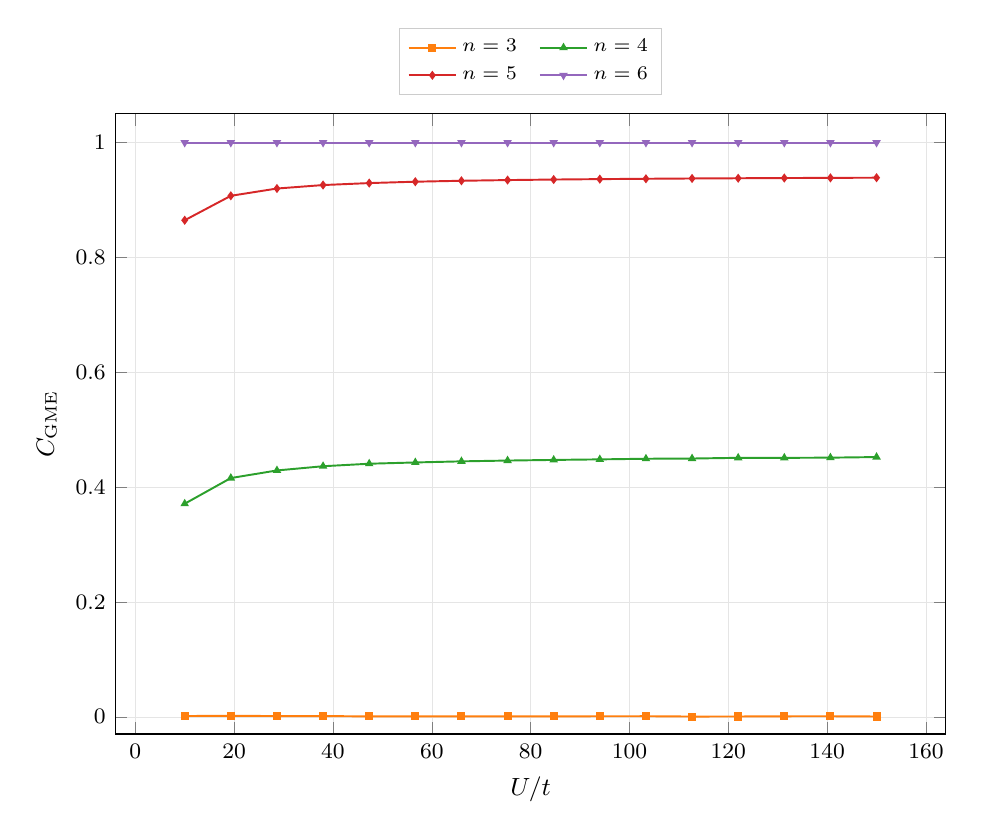
\begin{tikzpicture}
  \begin{axis}[
    width=\columnwidth,
    height=0.78\columnwidth,
    xlabel={$U/t$},
    ylabel={$C_{\mathrm{GME}}$},
    grid=both,
    grid style={line width=.1pt, draw=gray!20},
    tick label style={font=\footnotesize\rmfamily, /pgf/number format/fixed},
    label style={font=\small\rmfamily},
    scaled ticks=false,
    legend style={font=\scriptsize\rmfamily, draw=gray!40, at={(0.5,1.03)}, anchor=south, /tikz/every even column/.append style={column sep=6pt}},
    legend cell align={left},
    legend columns=2,
    ymin=-0.03,
    ymax=1.05,
  ]
    \addplot[color=gmeC1, mark=square*, mark size=1.1pt, line width=0.7pt] coordinates {
        (10,0.001392) (19.333333,0.001665) (28.666667,0.001353) (38,0.001318)
        (47.333333,0.000676) (56.666667,0.000645) (66,0.000867) (75.333333,0.000783)
        (84.666667,0.000852) (94,0.000935) (103.333333,0.001042) (112.666667,0.000447)
        (122,0.000544) (131.333333,0.000909) (140.666667,0.000971) (150,0.000532)
    };
    \addlegendentry{$n=3$}
    \addplot[color=gmeC2, mark=triangle*, mark size=1.1pt, line width=0.7pt] coordinates {
        (10,0.371043) (19.333333,0.415796) (28.666667,0.429004) (38,0.436361)
        (47.333333,0.440726) (56.666667,0.442933) (66,0.444852) (75.333333,0.446241)
        (84.666667,0.447345) (94,0.448299) (103.333333,0.449383) (112.666667,0.44977)
        (122,0.450987) (131.333333,0.450957) (140.666667,0.451313) (150,0.452328)
    };
    \addlegendentry{$n=4$}
    \addplot[color=gmeC3, mark=diamond*, mark size=1.1pt, line width=0.7pt] coordinates {
        (10,0.864713) (19.333333,0.907294) (28.666667,0.919964) (38,0.926014)
        (47.333333,0.929453) (56.666667,0.931848) (66,0.933473) (75.333333,0.934679)
        (84.666667,0.93561) (94,0.93635) (103.333333,0.936952) (112.666667,0.937451)
        (122,0.937855) (131.333333,0.938217) (140.666667,0.938543) (150,0.938814)
    };
    \addlegendentry{$n=5$}
    \addplot[color=gmeC4, mark=triangle*, mark size=1.1pt, mark options={rotate=180}, line width=0.7pt] coordinates {
        (10,1) (19.333333,1) (28.666667,1) (38,1)
        (47.333333,1) (56.666667,1) (66,1) (75.333333,1)
        (84.666667,1) (94,1) (103.333333,1) (112.666667,1)
        (122,1) (131.333333,1) (140.666667,1) (150,1)
    };
    \addlegendentry{$n=6$}
  \end{axis}
\end{tikzpicture}
